%% LaTeX-Beamer template for KIT design
%% by Erik Burger, Christian Hammer
%% title picture by Klaus Krogmann
%%
%% version 2.1
%%
%% mostly compatible to KIT corporate design v2.0
%% http://intranet.kit.edu/gestaltungsrichtlinien.php
%%
%% Problems, bugs and comments to
%% burger@kit.edu

\documentclass[18pt]{beamer}

%% SLIDE FORMAT

% use 'beamerthemekit' for standard 4:3 ratio
% for widescreen slides (16:9), use 'beamerthemekitwide'

\usepackage{templates/beamerthemekit}
% \usepackage{templates/beamerthemekitwide}

%% TITLE PICTURE

% if a custom picture is to be used on the title page, copy it into the 'logos'
% directory, in the line below, replace 'mypicture' with the
% filename (without extension) and uncomment the following line
% (picture proportions: 63 : 20 for standard, 169 : 40 for wide
% *.eps format if you use latex+dvips+ps2pdf,
% *.jpg/*.png/*.pdf if you use pdflatex)

\titleimage{lhc}

%% TITLE LOGO

% for a custom logo on the front page, copy your file into the 'logos'
% directory, insert the filename in the line below and uncomment it

\titlelogo{scc_logo}

% (*.eps format if you use latex+dvips+ps2pdf,
% *.jpg/*.png/*.pdf if you use pdflatex)

%% TikZ INTEGRATION

% use these packages for PCM symbols and UML classes
% \usepackage{templates/tikzkit}
% \usepackage{templates/tikzuml}

% the presentation starts here
\usepackage{caption}
\usepackage{subcaption}

\usepackage{tikz}
\usepackage{pgfplots}

\setbeamercovered{invisible}  % non transparent overlay

\title[rootJS]{rootJS - Specification}
\subtitle{PSE - Software Engineering Practice}
\author{C. Wolff, M. Fr\"uh, S. Rajgopal, C. Haas, J. Schwabe, T. Beffart}
%\author{Christoph Wolff, Maxi Fr\"uh, Sachin Rajgopal, Christoph Haas, Jonas Schwabe, Theo Beffart}

\institute{Steinbuch Center for Computing}

% Bibliography

\usepackage[citestyle=authoryear,bibstyle=numeric,hyperref,backend=biber]{biblatex}
\addbibresource{resources/references.bib}
\bibhang1em

\begin{document}

% change the following line to "ngerman" for German style date and logos
\selectlanguage{english}

%title page
\begin{frame}
\titlepage
\end{frame}

\section{PSE}

\begin{frame}{About PSE}
	Praxis der Softwareentwicklung(PSE) = Software Engineering Practice
	\begin{itemize}
		\item Waterfall model
		 \begin{itemize} 
			\item Planing/definition
		\end{itemize}
		\item Functional specification
	\end{itemize}
\end{frame}
\chapter{Purpose}
\paragraph{Project Goal}
The goal of this project is to create Node.js\textsuperscript{\textregistered}\footnote{\url{https://nodejs.org/}} bindings for
ROOT\footnote{\url{https://root.cern.ch/}}, thanks to which it will become possible to e.g. integrate ROOT into Node-based Web applications.\\
We aim specifically at ROOT 6 because its LLVM-based C++ interpreter Cling offers many advantages over the one available in older ROOT versions.
\section{Required criteria}
The bindings should:
\begin{itemize}
	\item work on Linux
	\item allow the user to interact with any ROOT class from the Node.js JavaScript interpreter
	\item accept C++ code for just-in-time compilation
	\item update dynamically following changes to C++ internals
	\item provide asynchronous wrappers for common I/O operations (i.e. file and tree access)
\end{itemize}
\pagebreak[3]

\section{Optional criteria}
The bindings should:
\begin{itemize}
	\item support the streaming of data in JSON format compatible with JavaScript ROOT
	\item implement a webserver based on node.js to mimic the function of the Root HTTP server
	\item work OS independent (i.e. support Mac OS X, Windows, Linux operating systems)
\end{itemize}

\section{Limiting criteria}
The bindings should not:
\begin{itemize}
	\item add any extending functionality to the existing ROOT framework
	\item necessarily support previous ROOT versions
	\item necessarily support future ROOT versions
\end{itemize}

\chapter{Product usage}

rootJS will be used to create web-applications that can:
\begin{itemize}
	\item Expose processed data (that might otherwise be hard to access) and then visualize it locally
	\item Interact with data both stored somewhere accessible for the server or streamed via remote procedure call (RPC)
	\item Run on any platform that supports a browser
\end{itemize}


\section{Audience}
Most users of rootJS will be used to working in Linux and with web servers. At the very least, they will be able to install ROOT
and also be proficient in programming languages like JavaScript and C++.
\begin{itemize}
	\item Scientists (e.g. particle physicists)
	\item Researchers
	\item Web-developers interested in creating applications based on ROOT
\end{itemize}

\section{Operating conditions}

rootJS will be used on servers that run ROOT and have access to the required data sources. As ROOT 6 currently runs on Linux and OS X only, usage of the bindings is limited to those platforms.

\chapter{Product environment}

\paragraph{Providing ROOT to node.js}\\
Node.js bindings for ROOT simplify the creation of server-client based ROOT applications. The bindings offer solutions based on state of the art web technology, especially the separation of data 
processing and visualization.

\section{Software}
\subsection{ROOT}
ROOT is a software framework for data analysis and I/O. It may be used to process and especially visualize big amounts of scientific data, e.g. the petabytes of data recorded by the Large Hadron Collider experiments every year.\\
Since the framework comes with an interpreter for the C++ programming language, for rapid and efficient prototyping and a persistency mechanism for C++ objects, ROOT based applications are  extensible and as feature rich as the C++ language itself.
A detailed introduction to the ROOT framework may be found in the \textit{ROOT  primer}\footnote[1]{\url{https://root.cern.ch/root/html534/guides/primer/ROOTPrimer.html}}
on the CERN website.\\
Interfacing with ROOT is done dynamically, since ROOT shares all the necessary information on its (global) functions during runtime.

\subsection{Node.js}
Node.js is an open source runtime environment. node.js is used to develop server-side web applications and may act as a 
stand alone webserver. It uses the Google V8 engine to execute the Javascript code. \\
The Binding API to be developed will be a so called native node.js module written in C++. It interfaces directly with the V8 API to provide (non-blocking) encapsulation of ROOT objects as Javascript equivalents.

\section{Hardware}
Since the Bindings, in simplified terms, just provide data structures for encapsulation of ROOT objects or rather functions, the hardware requirements of the bindings themselves should be negligible.\\
Basically calling a ROOT function via the Binding-API inside a node.js application really should not take up a huge amount of additional resources compared to a direct function call inside a native ROOT application.
In conclusion there are no additional hardware requirements for using the Bindings on a computer that was able to run native ROOT applications before - this includes almost any modern Desktop PC.

\chapter{Product data}

The following data will be stored by the rootJS bindings: \\

\begin{longtable}{|p{1cm} | p{15cm}|}
\hline
/D10/ & All ROOT classes and methods with corresponding signatures as they are dynamically mapped to JavaScript equivalents. They are also needed to support C/C++ specific features such as method overloading.\\
\hline
/D20/ & The ROOT environment state is preserved between calls from Node.js. This means that objects and variables are available until the rootJS session has ended or a reset was triggered explicitly.\\
\hline
/D30/ & The application context derived from \textit{TApplication}\footnotemark[1], storing at least the program name and path.\\
\hline
/D40/ & A map of \textit{v8::handle}'s\footnotemark[1] identified by the address of ROOT objects will be stored to allow proper handling of cyclic references, because the data is used to provide a cache that prevents stepping down in the recursive (object) creation endlessly.\\
\hline
\end{longtable}
\footnotetext[1]{{\url{root.api}}}
\chapter{Product interface and functions}
The rootJS bindings will not have a user interface, neither a graphical user interface nor a command line interface.
This section will therefore specify the API of rootJS.


\begin{longtable}{|p{1cm} | p{15cm}|}
   \hline
  /I10/ & The module will expose a JavaScript object containing all accessible root variables, functions and classes \\
  \hline
  /I20/ & Exposed variables might contain scalar values, in this case they will be accessible in their JavaScript counterparts \\
  \hline
  /I30/ & Exposed variables might be objects, which are recursively converted to JavaScript objects until there are only scalar values \\
  \hline
  /I40/ & Exposed variables might be enums. In this case the identifier of the currently selected value is returned instead of the corresponding integer \\
  \hline
  /I50/ & Every exposed method will be accessible via a proxy method which handles parameter overloading, as JavaScript does not support overloading. If there is no method to handle the passed arguments, an exception will be thrown \\
  \hline
  /I55/ & A method can be called with an additional callback method that will be called after the original method has been executed \\
  \hline
  /I60/ & Exposed classes will be accessible as a constructor returning the object. The constructor will be proxied to support parameter overloading. If there is no method to handle the passed arguments, an exception will be thrown  \\
  \hline
  /I65/ & A constructor can be called with an additional callback method that will be called after the object has been constructed \\
  \hline
  /I70/ & The classes are encapsulated in their namespaces from ROOT. Each namespace is an Object containing namespaces or class constructors \\
  \hline
  /I80/ & Exceptions thrown by Root will be forwarded to JavaScript and can be treated by JavaScript as normal exceptions \\
  \hline
  /I90/ & Global variables are accessible via getter and setter methods to ensure their values are kept in sync with the ROOT framework \\
   \hline
\end{longtable}

\section{Scenarios}

The bindings do not affect core functionality of ROOT. Therefore 
we decided to give some examples on how the bindings might be used. The 
user in this case is a Node.js based application, that uses the rootJS bindings 
to interact with ROOT. As the actual implementation is not yet 
finalized, the scenarios only contain samples of simple interactions 
between an Application and ROOT.

\subsection{Web Viewer Scenario}
\begin{figure}[htb]
	\centering
	\begin{longtable}{p{3cm} @{\hskip 1cm} p{12cm}}
		\hline
		
		\textit{Scenario Name} & \underline{WebViewer}\\
		\hline
	
		\textit{Abstract} & A browser based GUI for realtime representation of root graphs.\\
		\hline
	
		\textit{Participating actor instances} & \underline{WebViewer:Node.js}; \underline{:ROOT}; \underline{:rootJS}\\
		\hline
	
		\textit{Flow of events} & 
		\begin{enumerate}
			\item rootJS is up and running initialize has already been executed.
			
			\item WebViewer calls the API method to get graphical output of the data ROOT has currently loaded.
				\begin{enumerate}
					\item rootJS processes the request and calls the corresponding ROOT functionality.
					\item rootJS receives ROOT output and streams it to WebViewer.
				\end{enumerate}
			\item WebViewer uses the provided data to display the graph on its GUI.
				\begin{enumerate}
					\item Node.js invokes ROOT I/O operations.
						\begin{enumerate}
							\item ROOT loads data and provides raw visualization data.
						\end{enumerate}
					\item Node.js serializes data and streams it to WebViewer.
				\end{enumerate}
			\item WebViewer receives data and renders it in the browser.
		\end{enumerate}
		\\
		\hline
		
	\end{longtable}
	
	\caption{WebViewer scenario}
	
\end{figure}

\pagebreak[4]

\subsection{Event Viewer Scenario}
\begin{figure}[htb]
	\centering
	\begin{longtable}{p{3cm} @{\hskip 1cm} p{12cm}}
		\hline
		\textit{Scenario Name} & \underline{EventViewer}\\
		\hline
		\textit{Abstract} &
		A Web based event viewer providing a visualisation of experimental data, showing signals particles have produced in the detector.
		The web viewer is split into the back-end, server part, with access to
	    the data source and enough resources to process the data, and the front-end, client part, that is a modern-enough Web browser, and responsible only for visualisation itself and interaction with the user.
		\\
		\hline
		\textit{Participating actor instances} & 
		\underline{Server:Node.js Application}; \underline{:ROOT}; \underline{EventViewer:Browser}; \underline{:rootJS}\\
		\hline
		\textit{Flow of events} &
		\begin{enumerate}
			\item EventViewer requests visual updates from Server.
			\item Server interfaces with ROOT via rootJS.
			\item ROOT acquires data from external source.
			\begin{enumerate}
					\item External, dedicated readout hardware is used to access the data source.
					\item ROOT processes incoming data in a timely manner.
			\end{enumerate}
			\item ROOT passes the data prepared for (3D) visualisation to the Server via rootJS.
			\item Server publishes its data as JSON stream over the web.
			\item EventViewer renders received data locally e.g. using WebGL.
		\end{enumerate}
		\\
		\hline
	\end{longtable}
	\caption{EventViewer scenario}
\end{figure}

\section{Use Cases}

\subsection{UseROOTGlobal}
\begin{frame}{UseROOTGlobal}
        \begin{longtable}{p{3cm} @{\hskip 1cm} p{7cm}}
                \hline

                \textit{Use case name} & \texttt{UseROOTGlobal}\\
                \hline

                \textit{Participating actor instances} & Initiated by \texttt{NodeJSApplication}; Processed by \texttt{rootJS}; Communicates with \texttt{ROOT}\\
                \hline
                \pause

                \textit{Flow of events} &
                        \begin{enumerate}
                                \item The \texttt{NodeJSApplication} requests access to a global variable of \texttt{ROOT}.
                                \pause
                                \item \texttt{rootJS} sends a request to the corresponding \texttt{ROOT} variable.
                                \pause
                                \item \texttt{ROOT} returns the requested variable value.
                                \pause
                                \item The value is passed from \texttt{rootJS} to the \texttt{NodeJSApplication}.
                        \end{enumerate}
                        \\
        \end{longtable}
\end{frame}
\begin{frame}[t]{UseROOTGlobal}
        \begin{longtable}{p{3cm} @{\hskip 1cm} p{7cm}}
                \hline

                \textit{Entry condition} & \texttt{rootJS} has been initialized.\\
                \hline

                \textit{Exit condition} & The value has been returned to the \texttt{NodeJSApplication}.\\
                \hline
        \end{longtable}
\end{frame}

\subsection{UseROOTObject}
\begin{frame}{UseROOTObject}
        \begin{longtable}{p{3cm} @{\hskip 1cm} p{7cm}}
                \hline

                \textit{Use case name} & \texttt{UseROOTObject}\\
                \hline

                \textit{Participating actor instances} &
                Initiated by \texttt{NodeJSApplication}; Processed by \texttt{rootJS}, \texttt{ProxyObject}; Communicates with \texttt{ROOT}\\
                \hline
                                \pause

                \textit{Flow of events} &
                        \begin{enumerate}
                                \item The \texttt{NodeJSApplication} requests access to a \texttt{ROOT} object by calling a constructor function.
                                \pause
                                \item \texttt{rootJS} encapsulates the requested \texttt{ROOT} object within a \texttt{ProxyObject} that was created recursively.
                        \end{enumerate}
                        \\
        \end{longtable}
\end{frame}
\begin{frame}[t]{UseROOTObject}
        \begin{longtable}{p{3cm} @{\hskip 1cm} p{7cm}}
                \textit{Flow of events} &
                        \begin{enumerate}
                                \setcounter{enumi}{2}
                                \item \texttt{rootJS} stores the created \texttt{ProxyObject} in a cache memory.
                                \pause
                                \item The \texttt{ProxyObject} is exposed to the \texttt{NodeJSApplication}.
                        \end{enumerate}
                        \\
                \hline

                \textit{Entry condition} & \texttt{rootJS} has been initialized.\\
                \hline

                \textit{Exit condition} & The reference of the \texttt{ProxyObject} has been return to the \texttt{NodeJSApplication}.\\
                \hline
        \end{longtable}
\end{frame}

\subsection{UseROOTFunction}
\begin{frame}{UseROOTFunction}
        \begin{longtable}{p{3cm} @{\hskip 1cm} p{7cm}}
                \hline

                \textit{Use case name} & \texttt{UseROOTFunction}\\
                \hline

                \textit{Participating actor instances} & Initiated by \texttt{NodeJSApplication}; Processed by \texttt{rootJS}, \texttt{ProxyObject}; Communicates with \texttt{ROOT}\\
                \hline
                                \pause

                \textit{Flow of events} &
                        \begin{enumerate}
                                \item The \texttt{NodeJSApplication} requests access to a \texttt{ROOT} function.
                                \pause
                                \item \texttt{rootJS} calls the corresponding \texttt{ROOT} function.
                                \pause
                                \item \texttt{ROOT} responds.
                        \end{enumerate}
                        \\
        \end{longtable}
\end{frame}
\begin{frame}[t]{UseROOTFunction}
        \begin{longtable}{p{3cm} @{\hskip 1cm} p{7cm}}
                \textit{Flow of events} &
                        \begin{enumerate}
                                \setcounter{enumi}{3}
                                \item \texttt{rootJS} encapsulates the returned \texttt{ROOT} object within a \texttt{ProxyObject}.
                                \pause
                                \item The \texttt{ProxyObject} is exposed to the \texttt{NodeJSApplication}.
                        \end{enumerate}
                       \\
                \hline

                \textit{Entry condition} & \texttt{rootJS} has been initialized.\\
                \hline

                \textit{Exit condition} & The reference of the \texttt{ProxyObject} has been return to the \texttt{NodeJSApplication}.\\
                \hline
        \end{longtable}
\end{frame}

\subsection{UseJIT}
\begin{frame}{UseJIT}
        \begin{longtable}{p{3cm} @{\hskip 1cm} p{7cm}}
                \hline

                \textit{Use Case name} & \texttt{UseJIT}\\
                \hline

                \textit{Participating actor instances} & Initiated by \texttt{NodeJSApplication}; Processed by \texttt{rootJS}, \texttt{Cling}; Communicates with \texttt{ROOT}\\
                \hline
                                \pause

                \textit{Flow of events} &
                        \begin{enumerate}
                                \item The \texttt{NodeJSApplication} wants to execute \texttt{ROOT} specific C++ code (given as string) during runtime.
                                \pause
                                \item \texttt{rootJS} forwards the instructions to \texttt{Cling}.
                                \pause
                                \item \texttt{Cling} evaluates the received instructions using JIT compilation concepts and dynamically modifies the state of \texttt{ROOT}.
                        \end{enumerate}
                        \\
        \end{longtable}
\end{frame}
\begin{frame}[t]{UseJIT}
        \begin{longtable}{p{3cm} @{\hskip 1cm} p{7cm}}
                \textit{Flow of events} &
                        \begin{enumerate}
                                \setcounter{enumi}{2}
                                \item \texttt{rootJS} takes care of encapsulating exceptions possibly thrown by \texttt{Cling} or \texttt{ROOT} during evaluation and execution.
                                \pause
                                \item \texttt{rootJS} provides the evaluation results and corresponding return values to the \texttt{NodeJSApplication}.
                        \end{enumerate}
                        \\
                \hline

                \textit{Entry condition} & \texttt{rootJS} and \texttt{Cling} have been initialized.\\
                \hline

                \textit{Exit condition} & \texttt{rootJS} either confirms the proper execution of the specified instructions or forwards thrown exceptions to the \texttt{NodeJSApplication}.\\
                \hline
        \end{longtable}
\end{frame}

\section{System Model}
\subsection{Initialization}
\begin{frame}{Initialization}
  \begin{itemize}
    \item Expose all
    \begin{itemize}
      \item Global variables
      \item Global functions
      \item Classes
    \end{itemize}
    \pause
    \item Each are bound to corresponding proxy methods
    \item An object which members are the exposed features is beeing passed to node
  \end{itemize}
  \pause
  \begin{block}{Names}
    \begin{itemize}
      \item Functions and classes have the same name as in Root
      \item Global variables can be called using Get[Variable] and Set[Variable] methods
    \end{itemize}
  \end{block}
\end{frame}

\subsection{Call a feature}
\begin{frame}{Call a feature}
  \begin{itemize}
    \item All features in node are mapped to a proxy method that will be called
    \pause
    \item The proxy method will eventually call a root function and pass the result to our ObjectFactory
    \pause
    \item By looking at the object type an corresponding v8::Handle will be generated and returned to node
    \begin{itemize}
      \item If the result is an object this will be done recursively
    \end{itemize}
  \end{itemize}
\end{frame}

\chapter{Global Test Cases}
During the development process we will use continuous integration tools, running at least the following test cases: \\

\begin{longtable}{|p{1cm} | p{15cm}|}
  \hline
  /T10/ & Read all global variables \\
  \hline
  /T20/ & Write to all global variables that are not constant \\
  \hline
  /T30/ & Write to all global variables that are constant and ensure the correct Exception is thrown \\
  \hline
  /T40/ & Create instances of all classes with a public constructor \\
  \hline
  /T50/ & Call all methods of these Objects with valid parameters, where valid means that the 	data type is correct, a method throwing an exception due to invalid input shall be considered a passed test, a crash due to e.g. invalid memory read shall be considered a fail \\
  \hline
  /T60/ & Read all public member variables of these classes \\
  \hline
  /T70/ & Write to all public member variables of these classes that are not constant \\
  \hline
  /T80/ & Write to all public member variables of these classes that are constant and ensure the correct exception is thrown \\
  \hline
  /T90/ & Create instances of classes with private constructors and ensure the correct Exception is thrown \\
  \hline
  /T100/ &  The same for static members and methods \\
   \hline
\end{longtable}

\section{Statistics}

\begin{frame}{Merges}
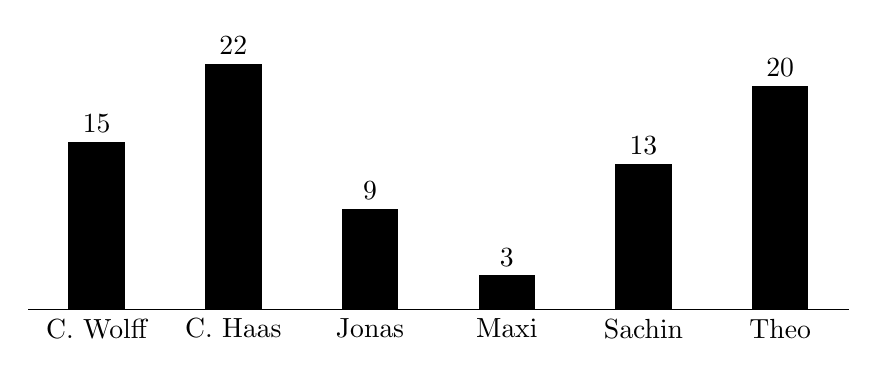
\begin{tikzpicture}
\begin{axis}[
     width  = 12cm,
     hide y axis,
     axis x line*=bottom,
     height = 5cm,
     bar width=20pt,
     symbolic x coords={C. Wolff, C. Haas, Jonas, Maxi, Sachin, Theo},
     nodes near coords,
     ymin=0
     ]
     \addplot[ybar, fill=black] coordinates {
          (C. Wolff,15)
          (C. Haas,22)
          (Jonas,9)
          (Maxi,3)
          (Sachin,13)
          (Theo,20)
     };
\end{axis}
\end{tikzpicture}
\end{frame}


\appendix
\beginbackup

\begin{frame}[allowframebreaks]{References}
\printbibliography
\end{frame}

\backupend

\end{document}
